\begin{FPfigure}

\begin{center}
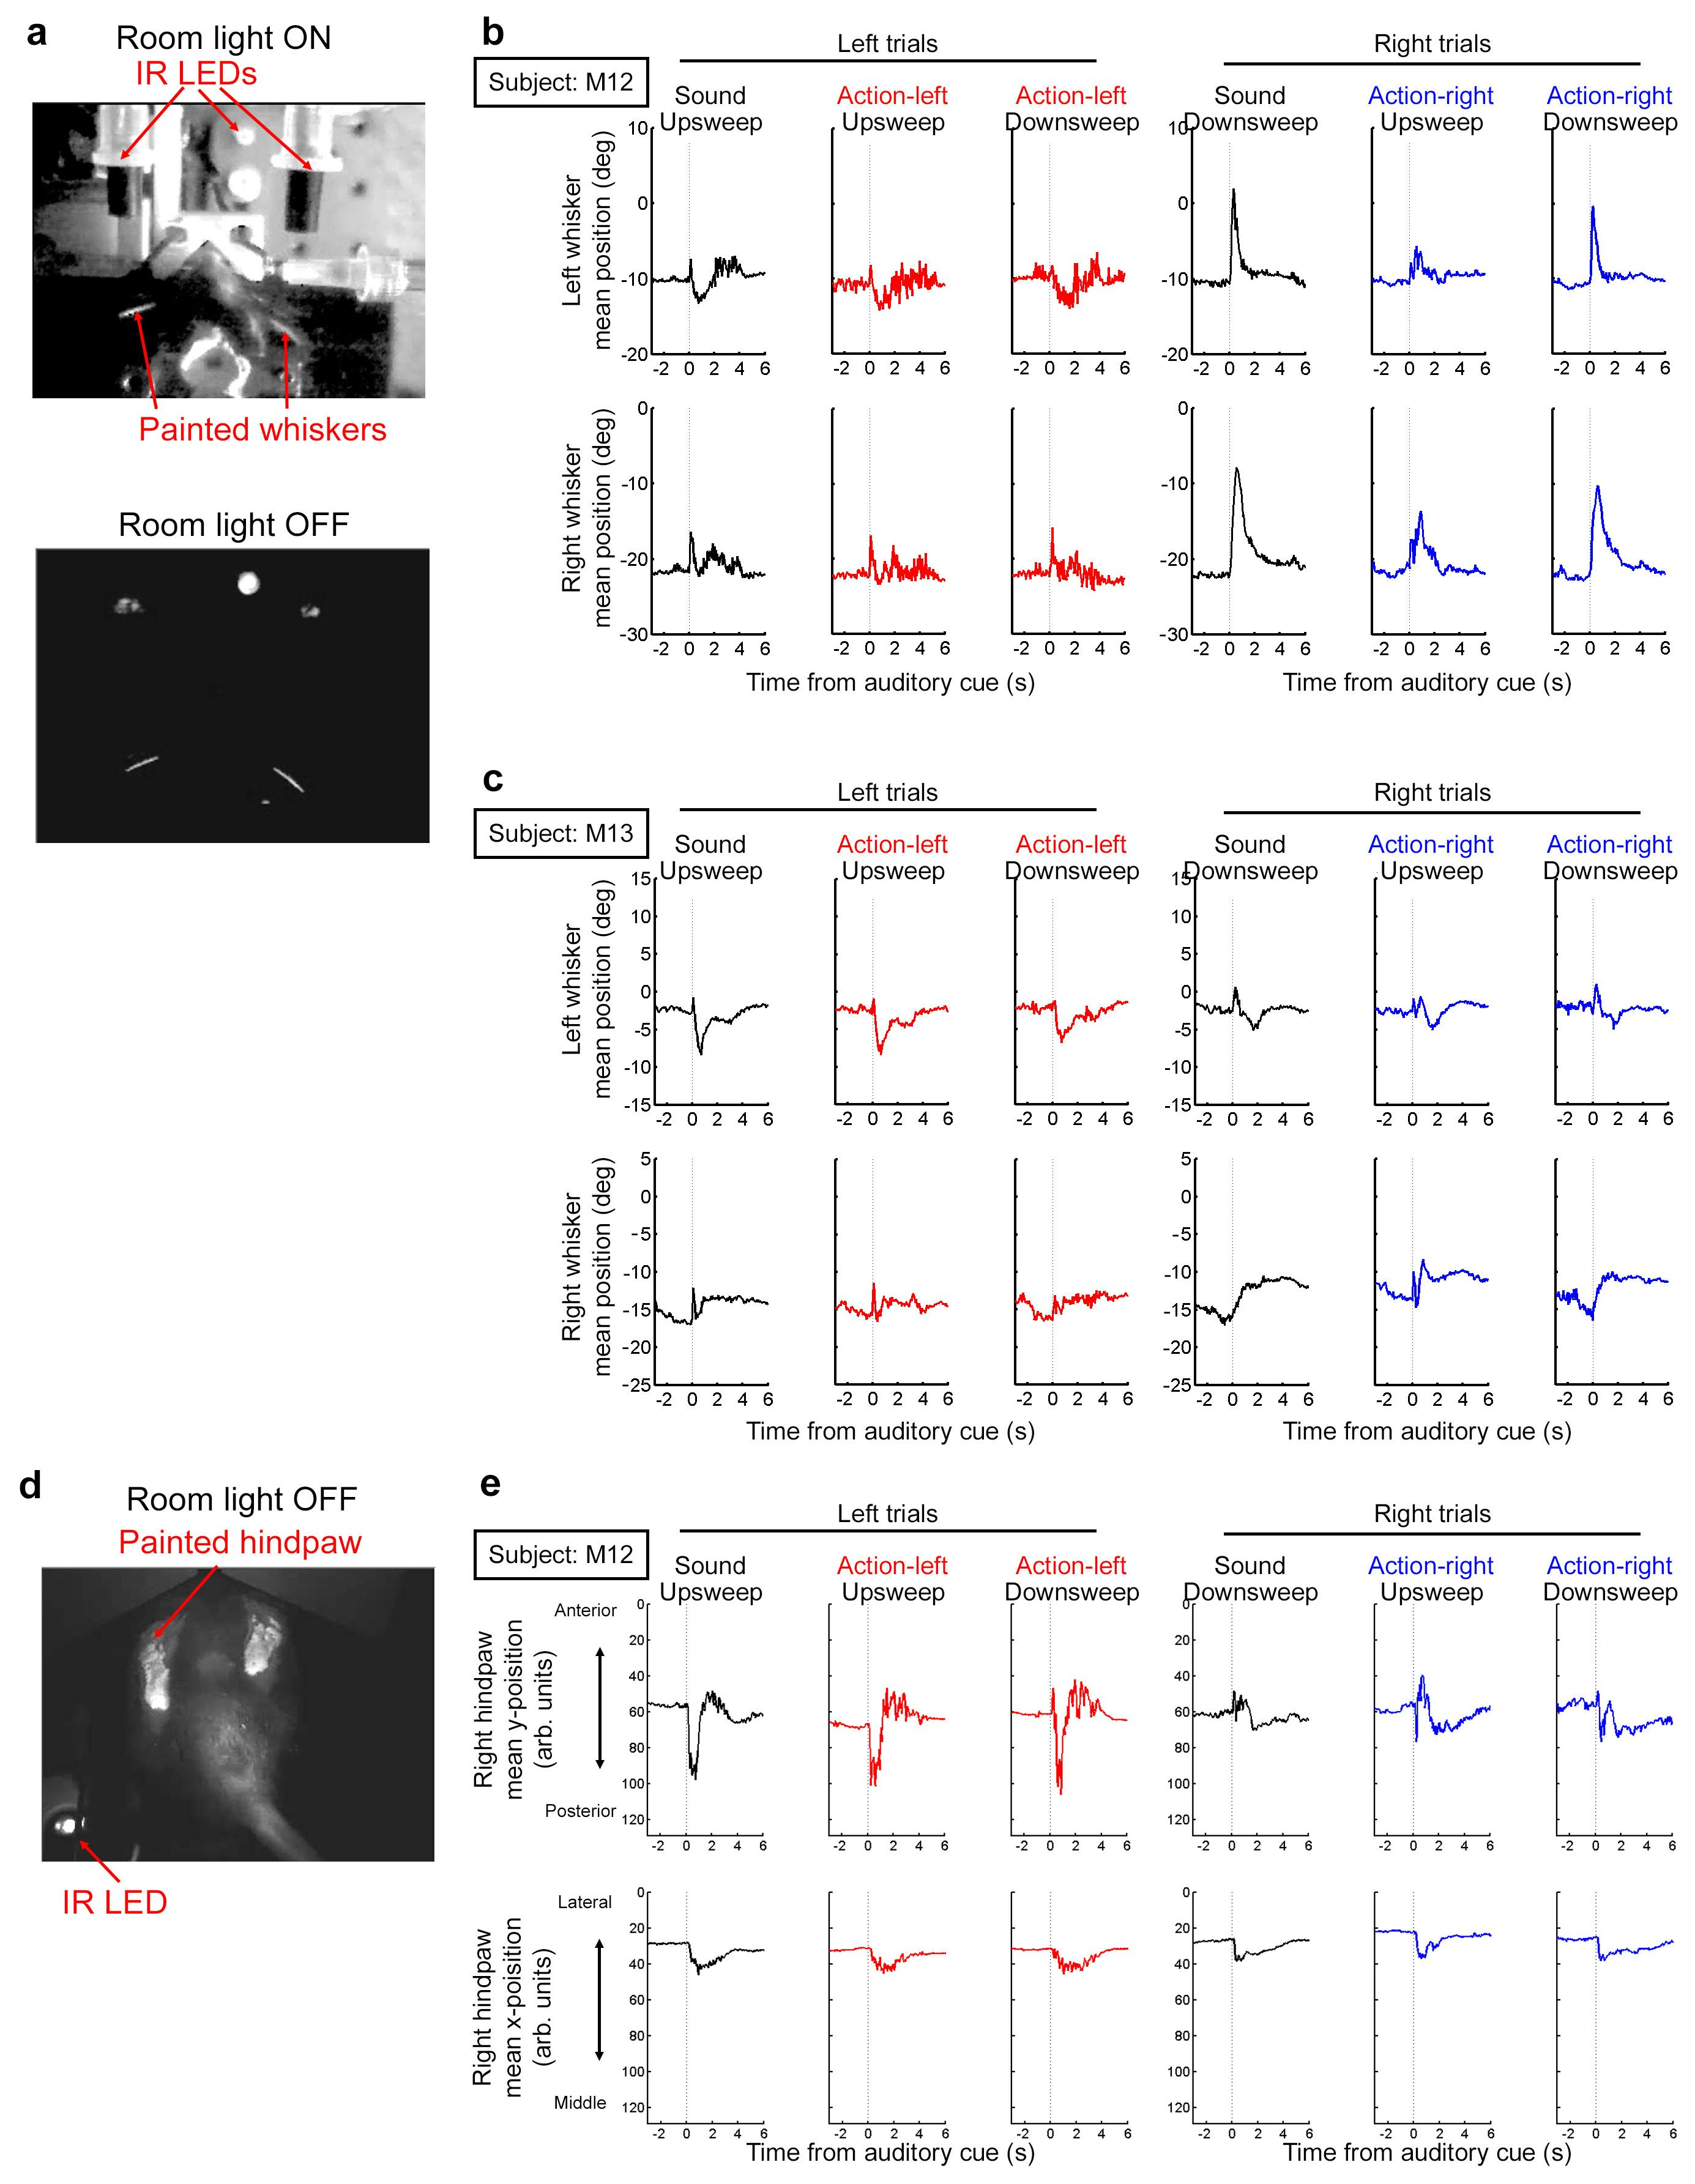
\includegraphics[width=\textwidth]{Figures/Chapter3/NN_figS3.jpg} 
\end{center}

\footnotesize{Supplementary Figure \ref{fig:NN_figS3}: Video tracking of whisker and hindpaw positions during the adaptive decision-making task.}

\caption[Video tracking of whisker and hindpaw positions during the adaptive decision-making task]
{Video tracking of whisker and hindpaw positions during the adaptive decision-making task. (a) Still frame from a video taken using an infrared webcam. One whisker on each side of the face was painted using a phosphorescent paint marker (cat. \#222-C-GO, Marvy Uchida). Whiskers were illuminated by two infrared light-emitting diodes (IR-LED). A third IR-LED was programmed to turn on 1 s before auditory cues, so the video could be synchronized to the task events. When the room light was turned off, the reflected infrared light could be visualized by the webcam. (b) Mean position of the left and right whiskers in different trial conditions for subject M12. These traces were averaged across correct trials within the last 20 trials pre-switch. For this analysis, each whisker was converted to a binary mask based on pixel intensity. The centroid of the mask was located in each frame, and then a line was fitted between the centroid and a fixed point on the face. The angle between the fitted line and the horizontal axis is reported, with positive deflections being protractions and negative deflections being retractions of the whisker. (c) Same as \emph{b} for another subject, M13. (d) Still frame from a video showing a painted hindpaw. The webcam was positioned under the animal, to record footage through the acrylic tube. The synchronization IR-LED is visible. (e) Mean x- and y- positions of the right hindpaw for different trial conditions for subject M12. Hindpaw and whisker data were obtained from two different behavioral sessions.}


\label{fig:NN_figS3}
\end{FPfigure}